\documentclass{beamer}

\usepackage[utf8]{inputenc} % Language and font encoding
\usepackage[icelandic]{babel}
\usepackage[T1]{fontenc}


\usepackage{tikz}
\usepackage[listings,theorems]{tcolorbox}
\usepackage{booktabs}
\usepackage{minted} %Minted and configuration
\usemintedstyle{default}

\renewcommand{\theFancyVerbLine}{\sffamily \arabic{FancyVerbLine}}
%%%%%%%%%%%
% More math
%%%%%%%%%%%
\newcommand{\Mod}[1]{\ \text{mod}\ #1}

%%%%%%%%%%%%%%%%%%%%%%
% Beamer configuration
%%%%%%%%%%%%%%%%%%%%%%
\setbeamertemplate{navigation symbols}{}
\usecolortheme{dove}
\setbeamercolor{frametitle}{fg=white}

\usebackgroundtemplate%
{%
\vbox to \paperheight{

\includegraphics[width=\paperwidth]{Pics/hi-slide-head-2016}

\vfill
\hspace{0.5cm}
\includegraphics[width=0.3\paperwidth]{Pics/hi-von-logo}
\vspace{0.4cm}
    }%
}

\AtBeginSection[]
{
  \begin{frame}<beamer>
    \frametitle{Yfirlit}
    \tableofcontents[currentsection]
  \end{frame}
}

\setbeamerfont{frametitle}{size=\normalsize}
\addtobeamertemplate{frametitle}{}{\vspace*{0.5cm}}

%%%%%%%%%%%%%%%%%%%%%%%%%
% tcolorbox configuration
%%%%%%%%%%%%%%%%%%%%%%%%%

% Setup from: http://tex.stackexchange.com/a/43329/21638
\tcbset{%
    noparskip,
    colback=gray!10, %background color of the box
    colframe=gray!40, %color of frame and title background
    coltext=black, %color of body text
    coltitle=black, %color of title text 
    fonttitle=\bfseries,
    alerted/.style={coltitle=red, colframe=gray!40},
    example/.style={coltitle=black, colframe=green!20, colback=green!5},
}


%%%%%%%%%%%%%%%%%%%%%%%
% Further configuration
%%%%%%%%%%%%%%%%%%%%%%%
\hypersetup{colorlinks=true,pdfauthor={Eirikur Ernir Thorsteinsson},linkcolor=blue,urlcolor=blue}
\graphicspath{{./Pics/}}

\author{Eiríkur Ernir Þorsteinsson}
\institute{Háskóli Íslands}
\date{Haust 2016}

\usetikzlibrary{automata,positioning}

\title{Stærðfræðimynstur í tölvunarfræði}
\subtitle{Vika 14, fyrri fyrirlestur}

\begin{document}

\begin{frame}
\titlepage
\end{frame}


\section{Inngangur}

\begin{frame}{Í síðasta tíma}
\begin{itemize}
 \item Endanlegar stöðuvélar
 \begin{itemize}
  \item \ldots með úttaki
  \item \ldots án úttaks
 \end{itemize}
\end{itemize}
\end{frame}

\begin{frame}{Planið}
\begin{itemize}
 \item Í dag: Turing-vélar + stoðtími
 \item Í dæmatímum: Skiladæmi síðustu viku + spurningar um námsefni misserisins
 \item Á föstudaginn: Skiladæmi þessarar viku + spurningar um námsefni misserisins
\end{itemize}
\end{frame}


\section{Turing-vélar}

\begin{frame}{Takmarkanir endanlegra stöðuvéla}
\begin{itemize}
 \item Endanlegar stöðuvélar geta ekki leyst öll okkar vandamál
 \item Dæmi um vandamál sem ekki er leysanlegt með endanlegri stöðuvél - þekkja málið $\{0^n1^n | n\geq 0\}$
 \begin{itemize}
  \item Hvað myndum við þurfa margar stöður til að þekkja það?
 \end{itemize}
 \item Innleiðum nýja gerð af vél - Turing vél
 \begin{itemize}
  \item Nefndar eftir Alan Turing, sem kallaði þær a-vélar (``Automatic machine'')
 \end{itemize}
\end{itemize}
\end{frame}

\begin{frame}{Turing vél}
Lykilatriði í Turing vélum: Stöður, ``hausinn'' og ``bandið''. Svipar til hugmyndarinnar um les- og skrifhaus á segulbandi.
\begin{center}
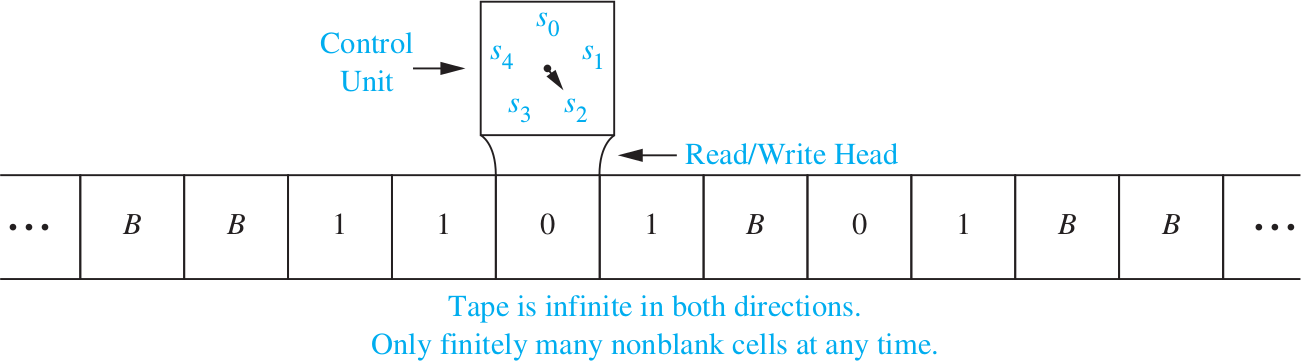
\includegraphics[width=\textwidth]{turing-machine-example1}
\end{center}
\end{frame}

\begin{frame}{Skilgreining}
\begin{tcolorbox}[title=Turing vél]
Turing vél $T = (S, I, f, s_0)$ samanstendur af
\begin{itemize}
 \item $S$, mengi af stöðum
 \item $I$, stafróf sem inniheldur ``tómt tákn'' $B$
 \item $f$, hlutskilgreint fall $f$ frá $S \times I$ til $S \times I \times \{L, R\}$
 \item $s_0$, upphafsstöðu
\end{itemize}
\end{tcolorbox}
Þessi vél vinnur á óendanlegu ``bandi'' (e. \emph{tape}) sem í upphafi inniheldur endanlegan fjölda tákna sem eru ekki tóm. Bandinu er skipt niður í hólf. Líkt og fyrir endanlegar stöðuvélar getum við líka skilgreint lokastöður.
\end{frame}

\begin{frame}{Keyrsla Turing vélar}
\begin{itemize}
 \item Látum vélina vera í stöðu $s$, með leshausinn á tákni $x$
 \item Sé $f(s,x) = (s',x',d)$ skilgreint gerum við eftirfarandi:
 \begin{enumerate}
  \item Færum vélina í stöðu $s'$
  \item Skrifum $x'$ í hólfið þar sem leshausinn er staðsettur ($x$ er yfirskrifað)
  \item Færum leshausinn eitt hólf til vinstri ef $d = L$, en eitt hólf til hægri ef $d = R$
 \end{enumerate}
 \item Sé $f$ ekki skilgreint fyrir parið $(s,x)$ stöðvast vélin
 \item Getum lýst Turing-vél með mengi $5$-unda, hver þeirra á sniðinu:
\end{itemize}
\[(s, x, s' , x' , d)\]
\end{frame}

\begin{frame}{Dæmi}
\begin{columns}
\column{0.4\textwidth}
\begin{itemize}
 \item Skilgreinum Turing vél með $5$-undum
 \begin{itemize}
  \item $(s_0 , 0, s_0 , 0, R)$
  \item $(s_0 , 1, s_1 , 1, R)$
  \item $(s_0 , B, s_3 , B, R)$
  \item $(s_1 , 0, s_0 , 0, R)$
  \item $(s_1 , 1, s_2 , 0, L)$
  \item $(s_1 , B, s_3 , B, R)$
  \item $(s_2 , 1, s_3 , 0, R)$
 \end{itemize}
 \item og keyrum hana á bandinu til hægri
\end{itemize}
\column{0.6\textwidth}
\begin{center}
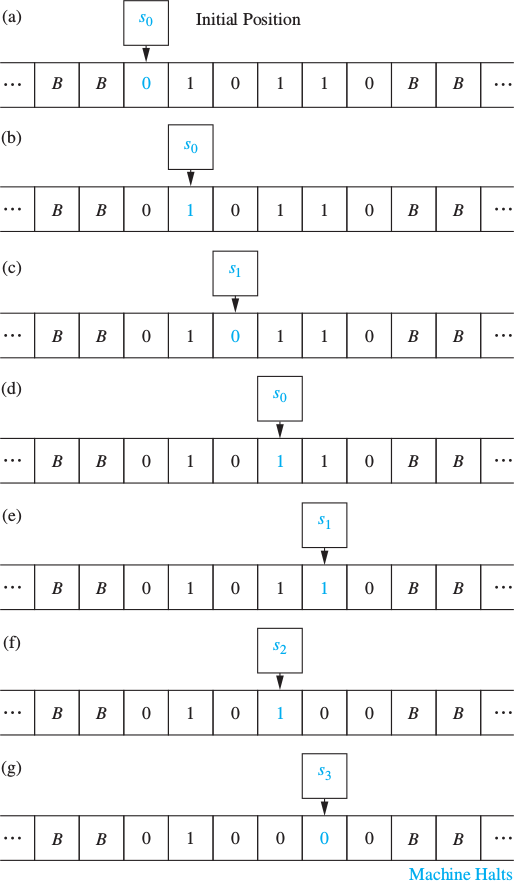
\includegraphics[width=0.7\textwidth]{turing-machine-example2}
\end{center}
\end{columns}
\end{frame}

\section{Turing vélar og mál}

\begin{frame}{Mál}
Við getum látið Turing-vélar samþykkja strengi og mál.

\begin{tcolorbox}
Látum $V$ vera hlutmengi stafrófs $I$. Turing vél $T$ með lokastöðum samþykkir streng $x \in V^*$ ef $T$ stöðvast í lokastöðu þegar $x$ er skrifaður á bandið og vélin sett í gang með hausinn á fyrsta tákninu í $x$. $T$ samþykkir málið $A \subseteq V^*$ ef $T$ samþykkir $x$ þá og því aðeins að $x$ tilheyri $A$.
\end{tcolorbox}

\end{frame}

\begin{frame}{Dæmi}
Smíðum Turing vél sem samþykkir mál þeirra strengja sem hafa $0$ sem bita númer 2.

\begin{center}
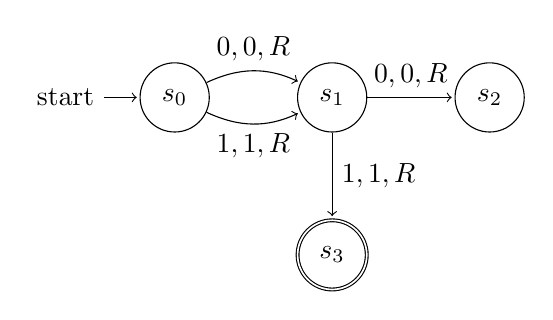
\begin{tikzpicture}[shorten >=1pt,node distance=2cm,on grid,auto] 
  \node[state,initial]		(s0) 			{$s_0$};
  \node[state]			(s1) [right = of s0]	{$s_1$};
  \node[state]			(s2) [right = of s1]	{$s_2$};
  \node[state, accepting]	(s3) [below = of s1]	{$s_3$};
  
  \path[->]
%   (s0) edge [align=center,loop above] node{loooop} ()
  (s0) edge [align=center, bend left = 25] node{$0, 0, R$} (s1)
  (s0) edge [align=center, bend right = 25, below] node{$1, 1, R$} (s1)
  (s1) edge [align=center] node{$0, 0, R$} (s2)
  (s1) edge [align=center, right] node{$1, 1, R$} (s3)
%   (s0) edge [align=center,bend left = 25,right] node{bend}(s1)
  ;
\end{tikzpicture}
\end{center}
\end{frame}

\begin{frame}{Dæmi}
Smíðum Turing vél sem samþykkir málið $\{0^n1^n | n \geq 1\}$.

\begin{center}
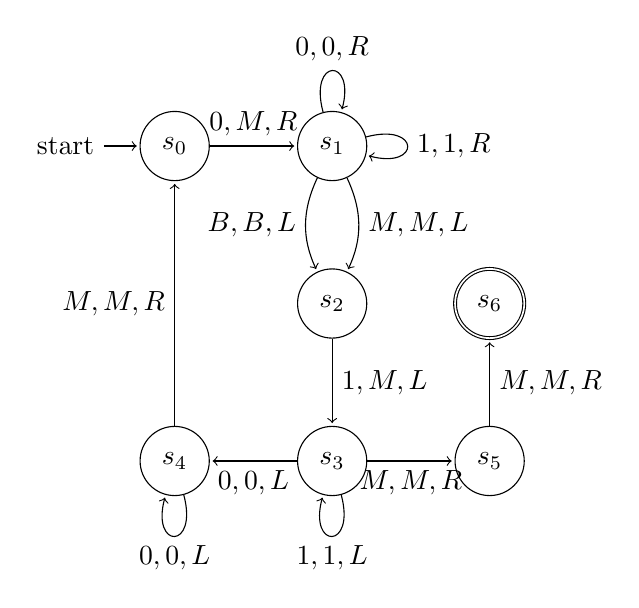
\begin{tikzpicture}[shorten >=1pt,node distance=2cm,on grid,auto] 
  \node[state,initial]		(s0) 			{$s_0$};
  \node[state]			(s1) [right = of s0]	{$s_1$};
  \node[state]			(s2) [below = of s1]	{$s_2$};
  \node[state]			(s3) [below = of s2]	{$s_3$};
  \node[state]			(s4) [left  = of s3]	{$s_4$};
  \node[state]			(s5) [right = of s3]	{$s_5$};
  \node[state, accepting]	(s6) [above = of s5]	{$s_6$};
 
  \path[->]
  (s0) edge [align=center] node{$0, M, R$} (s1)
  (s1) edge [align=center, loop above] node{$0,0,R$} () 
  (s1) edge [align=center, loop right] node{$1,1,R$} ()
  (s1) edge [align=center, bend left = 25, right] node{$M, M, L$} (s2)
  (s1) edge [align=center, bend right = 25, left] node{$B, B, L$} (s2)
  (s2) edge [align=center] node{$1, M, L$} (s3)
  (s3) edge [align=center, loop below] node{$1,1,L$} ()
  (s3) edge [align=center] node{$0, 0, L$} (s4)
  (s3) edge [align=center, below] node{$M, M, R$} (s5)
  (s4) edge [align=center, loop below] node{$0,0,L$} ()
  (s4) edge [align=center] node{$M, M, R$} (s0)
  (s5) edge [align=center, right] node{$M, M, R$} (s6)
  ;
\end{tikzpicture}
\end{center}
\end{frame}


\end{document}
